%%%% Proceedings format for most of ACM conferences (with the exceptions listed below) and all ICPS volumes.
\documentclass[sigconf]{acmart}

\usepackage{listings}
\usepackage{color}
\usepackage[htt]{hyphenat}

\definecolor{dkgreen}{rgb}{0,0.6,0}
\definecolor{gray}{rgb}{0.5,0.5,0.5}
\definecolor{mauve}{rgb}{0.58,0,0.82}

\lstset{frame=tb,language=Java,aboveskip=3mm,belowskip=3mm,showstringspaces=false,columns=flexible,basicstyle={\small\ttfamily},numbers=none,numberstyle=\tiny\color{gray},keywordstyle=\color{blue},commentstyle=\color{dkgreen},stringstyle=\color{mauve},breaklines=true,breakatwhitespace=true,tabsize=3}

\settopmatter{printacmref=false} % Removes citation information below abstract
\renewcommand\footnotetextcopyrightpermission[1]{} % removes footnote with conference information in first column
\pagestyle{plain} % removes running headers

%%%% As of March 2017, [siggraph] is no longer used. Please use sigconf (above) for SIGGRAPH conferences.

%%%% Proceedings format for SIGPLAN conferences 
% \documentclass[sigplan, anonymous, review]{acmart}

%%%% Proceedings format for SIGCHI conferences
% \documentclass[sigchi, review]{acmart}

%%%% To use the SIGCHI extended abstract template, please visit
% https://www.overleaf.com/read/zzzfqvkmrfzn


\usepackage{booktabs} % For formal tables


% Copyright
\setcopyright{none}
%\setcopyright{acmcopyright}
%\setcopyright{acmlicensed}
%\setcopyright{rightsretained}
%\setcopyright{usgov}
%\setcopyright{usgovmixed}
%\setcopyright{cagov}
%\setcopyright{cagovmixed}

\begin{document}
\title{SOEN7481 Fall 2018: Assignment}
\subtitle{Building a Bug Pattern Detector Tool\\\url{https://github.com/AdrienPoupa/soen7481-assignment}}

\author{Yann Kerichard}
\affiliation{%
  \institution{Concordia University}
  \city{Montreal}
  \state{Quebec}
  \country{Canada}
}

\author{Yousef Saatchi}
\affiliation{%
  \institution{Concordia University}
  \city{Montreal}
  \state{Quebec}
  \country{Canada}
}

\author{Gagandeep Kaur}
\affiliation{%
  \institution{Concordia University}
  \city{Montreal}
  \state{Quebec}
  \country{Canada}
}

\author{Gagandeep Singh}
\affiliation{%
  \institution{Concordia University}
  \city{Montreal}
  \state{Quebec}
  \country{Canada}
}

\author{Karanvir Singh Sidhu}
\affiliation{%
  \institution{Concordia University}
  \city{Montreal}
  \state{Quebec}
  \country{Canada}
}

\author{Adrien Poupa}
\affiliation{%
  \institution{Concordia University}
  \city{Montreal}
  \state{Quebec}
  \country{Canada}
}


\begin{abstract}
Bug detection is crucial is modern software, as it helps developers to find their mistakes and correct them. Bugs can be detected statically or dynamically. Static bug detection is done without running the code; it happens in Integrated Development Environment such as Eclipse or IntelliJ for example. On the other hand, dynamic bug detection is performed at runtime.\\In this study, we have created a Bug Pattern Detector, inspired by FindBugs \cite{findbugs} and SpotBugs \cite{spotbugs}, that can detect and classify bug patterns in ten different categories. Our parser is based on the JavaParser \cite{javaparser} open source library, that can parse Java files into abstract syntax trees. We have tested our solution by creating unit tests. We have run our tool on two open-source softwares: Hadoop 3.0.0 and CloudStack 4.9. We compared the results with FindBugs. 

\end{abstract}

\keywords{Bug Pattern, Java, Java Parser, jUnit, FindBugs}

\maketitle

\section{Introduction}
In a world that heavily relies on software, reliability is crucial. To ensure it, several approaches have been used: bug detection, whether static or dynamic, testing (unit testing, integration testing, etc), reviewing, and so on.\\To improve software reliability, we have created a static analysis tool that detects bug patterns in Java classes. We took inspiration from the open source software FindBugs \cite{findbugs} and its successor SpotBugs \cite{spotbugs}. We used the book "JavaParser: Visited" \cite{javaparservisited} to understand how the JavaParser \cite{javaparser} library that we used to parse Java files. Our software covers ten different bug patterns that consist of the following:
\begin{enumerate}
    \item \textit{Class defines \texttt{equals} but not \texttt{hashCode}}: if a class overrides the \texttt{equals} function but not the \texttt{hashCode} function, causing the \texttt{HashMap} and \texttt{HashSet} functions to fail;
    \item \textit{Comparison of \texttt{String} objects using == or !=}: Java uses the \texttt{equals} function to test the equality between two string, and not a double equal sign unlike other languages;
    \item \textit{Method may fail to close stream on exception}: when a stream is open, it should be closed in the finally block. Failing to do so may result in a file descriptor leak.
    \item \textit{Condition has no effect}: finds useless conditions that are always true or false, resulting in redundant code;
    \item \textit{Inadequate logging information in catch blocks}: logging the same information in different catch blocks can be confusing for the developer, can make debugging difficult and should not happen;
    \item \textit{Unneeded computation in loops}: some variables created inside a loop may not be used later, creating an unnecessary overhead;
    \item \textit{Unused methods}: functions that are not used create unneeded additional complexity and should be removed:
    \item \textit{Empty exception}: if there is no information displayed when an exception occurs, difficulties can arise when debugging the program;
    \item \textit{Unfinished exception handling code}: if there is a comment stating \texttt{TODO} or \texttt{FIXME} in the catch block of an exception, this means that the exception handling should be finished;
    \item \textit{Over-catching an exception with system-termination}: when developers are catching high levels exceptions such as Exception or \texttt{RuntimeException} and there is a call to \texttt{System.\-exit(0)} in the catch block of an exception, the programs halts and this behavior is not desired.
\end{enumerate}
We have created unit tests using the jUnit framework to ensure that those bugs were detected by our tool. Then, we tried our tool on two open-source softwares, Hadoop 3.0.0 and CloudStack 4.9, and we compared the results with FindBugs. We found that in some cases, our tool detected false positives that FindBugs did not and for some other cases, our tool detected bugs undetected by FindBugs.

\section{Detection Approach}
Our bug pattern detector relies on Java Parser, an open source library used to parse Java code.
\subsection{Project Architecture} At the root of our project, the \texttt{filesToParse} folder contains, as its name states, the files that are to be parsed by our tool. Then, following Maven's standard layout \cite{mavenlayout}, the java files are located in the \texttt{src} folder. Within this folder are the main and test directories, containing the project's sourcecode and the unit tests, respectively. The project can be run from the \texttt{Main} class, that acts as the driver. Alongside the \texttt{Main} class, the \texttt{Util} class contains the common functions used throughout the code (\texttt{getFunctionName} to get the name of a parent function from a \texttt{Node}, \texttt{getLineNumber} to get the line number of a given \texttt{Node}). The \texttt{FileUtil} class is reponsible for reading and writing the HTML report. Finally, the \texttt{DirExplorer} class handles the exploration of folders recursively.The \texttt{BugPattern} package contains the \texttt{Bug} interface that is implemented by the abstract \texttt{BugPattern} class. Then, each of the ten bug patterns extend the \texttt{BugPattern} class, overriding the \texttt{getIdentifier}, \texttt{getName} and \texttt{getDescription} methods used in the report.\\The \texttt{Checker} package contains the \texttt{Checker} interface that is implemented by the bug checkers classes, one for each bug pattern. Each checker defines the \texttt{check} function, used to search for a specific bug pattern in a given class. Figure \ref{uml} shows a package diagram for our solution. In listing \ref{lst:checker}, the common base for all the checkers is shown. Each checker relies on the Visitor pattern; we override the appropriate visitor function provided by the Java Parser library to collect the required information for the bug pattern, and when the requirements are met, we add the bug pattern into the list that we return at the end of the function. \texttt{DirExplorer} ensures that this is run for every file contained in the parsing folder.
\begin{lstlisting}[caption={Excerpt of the \texttt{check} function common to each checker},captionpos=b,label={lst:checker}]
public List<BugPattern> check(File projectDir) {
    List<BugPattern> bugPatterns = new ArrayList<>();

    new DirExplorer((level, path, file) -> path.endsWith(".java"), (level, path, file) -> {
        try {
            new VoidVisitorAdapter<Object>() {
                @Override
                // The prototype of the visit function that we override depends on the bug pattern that we want to implement
                public void visit(Node n, Object arg) {
                    super.visit(n, arg);
                    // Here is the specific code
                    ...
                    // When the conditions are met, add the bug pattern to the list
                    if (bug conditions are met) {
                        // Get the line number
                        int lineNumber = Util.getLineNumber(n);

                        // Get the method name
                        String functionName = Util.getFunctionName(n);

                        // Add the bug pattern to the list
                        bugPatterns.add(new BugPatternName(lineNumber, file, functionName));
                    }
                }
            }.visit(JavaParser.parse(file), null);
        } catch (IOException e) {
            new RuntimeException(e);
        }
    }).explore(projectDir);

    return bugPatterns;
}
\end{lstlisting}

\newpage
\noindent

\subsection{Generating the Report} Once all the checkers are executed and all the bug patterns are found, an HTML report is generated using a template. The report can be found in /results/report.html. An example of such a report is shown in figure \ref{report}. It gives a summary of the bug patterns found, and a detailed table that states where the bug was found (file name, line number) and which bug pattern it is.

\subsection{Bug Checkers Explanation}
\begin{enumerate}
    \item \textit{Class defines \texttt{equals()} but not \texttt{hashCode()}} is using a visitor object inspecting each method of the provided file. Then, for each of those methods, our tool will try to identify the name and the return type of the method. If this name is \textit{equals} and the return type is a Boolean, then a boolean value will be set to true, specifying that the equals method has been found. The tool also looks for a method named \textit{hashCode}, having for return type a string, and not having any arguments. If this method is found, another boolean value is set to true. Finally, if one of both boolean values is false, the tool indicates an error.
    \item \textit{Comparison of \texttt{String} objects using == or !=} uses 2 visitors objects. To implement this bug pattern detection, we decided to use an \texttt{HashMap} object to store all the variables of each class. First, thanks to the first visitor object, the tool will inspect each method of the file, in order to identify all String parameter's name. Then, a second visitor allows the tool to inspect each statement. In the case where the tool detects a line using an equal symbol with 2 string objects, we notify the user that a bug is detected.
    \item \textit{Method may fail to close stream on exception} will be identified thanks to a visitor object, inspecting all method declarations. The tool will then be able to detect many kinds of stream declaration statements. Each stream is stored in an \texttt{HashMap} object. If the tool detect a line with a \textit{close()} instruction, and if the object on which this instruction is executed is referenced in the stream's \texttt{HashMap}, the stream object is then removed. Finally, for each stream object still present in the \texttt{HashMap} at the end, an error message will be displayed.
    \item \textit{Condition has no effect} inspects each single line of code. If the tool detects a condition statement where the condition is a literal expression (such as true for example), an error message is displayed. The tool also handles the case where the condition is comparing two objects with the same name (such as \texttt{a = a}). An error is then displayed.
    \item \textit{Inadequate logging information in catch blocks} uses a visitor that only inspect each \texttt{Try} block statement. The error message is then stored in an ArrayList object. If the same error message appears twice, then, the tool will notify the user that there is an error.
    \item \textit{Unneeded computation in loop} implements a visitor pattern that visits all the kinds of loops and check for any variable declaration which are then added to a list. Then we iterate through each line of code recursively and check if the variable in the list is present in the line other than the place of their declaration. If found, that variable is removed from the list and at last each variable still present in the list its the line number and function name are fetched and added to the array list of \texttt {Bug Pattern}.  
    \item \textit{Unused methods} checker: Firstly. we check for \texttt{jUnit} importation in the class and if the method contains test annotation then it is not checked since test cases are never called directly from the source code. For rest of the methods they are added to the \texttt{hashMap} along with their class name. After that, we use visitor to visit each class and we iterate over \texttt{hashMap} to check if the current class contains the method in the \texttt{hashMap} then we set the flag for found variable to true and continue checking for other methods and if for some class, methods are not found in the \texttt{hashMap}, and also they are not a main method, then we set the flag to false and is added to to the array list of \texttt {Bug Pattern}.
    \item \textit{Empty exception} checker: we used the catch clause visitor to parse the code containing the catch clause. After that we get the body of the catch block in \texttt {Block Statement} object and using this object we fetched all the statements of the block in the \texttt {NodeList} object. If there exists no statement, then the line number from where the catch block is starting and its function name are fetched and added to the array list of \texttt {Bug Pattern}. 
    \item \textit{Unfinished exception handling code} checker: For implementing the checker, we used the catch clause visitor pattern to parse the code containing the catch clause. After that we iterate through all the comments contained in the catch block and if the comment contains \texttt {fixme} or \texttt{TODO} as a text then the line number of the comment and its function name are fetched and added to the arraylist of \texttt{Bug Pattern}.
    \item \textit{Over-catching an exception with system-termination} checker we used the catch clause visitor pattern to parse the code containing the catch clause and get its parameters. If the parameter contains any of the known exceptions then its body of catch block is fetched and from that we get the list of statements. After that we iterate through all the statements to get the values of \texttt{NameExpr} and \texttt{MethodCallExpr} and if they match with system and exit respectively we get the function name and its line number to add to the array list of \texttt {Bug Pattern}.

\end{enumerate}

\begin{figure}
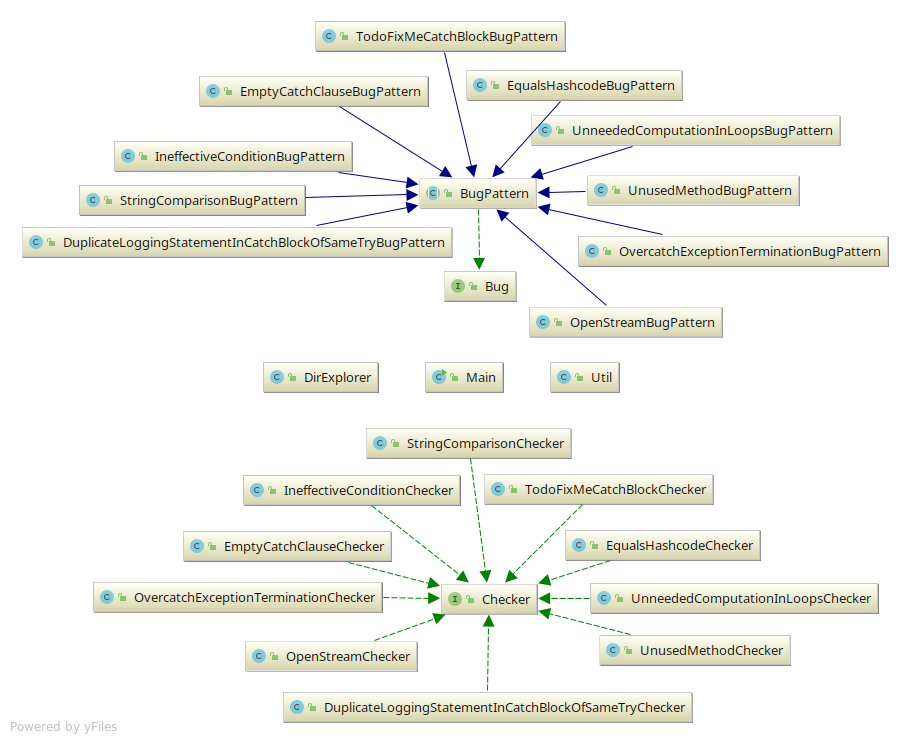
\includegraphics[width=0.5\textwidth]{uml}
\caption{UML Package Diagram of our tool}
\label{uml}
\end{figure}

\begin{figure}
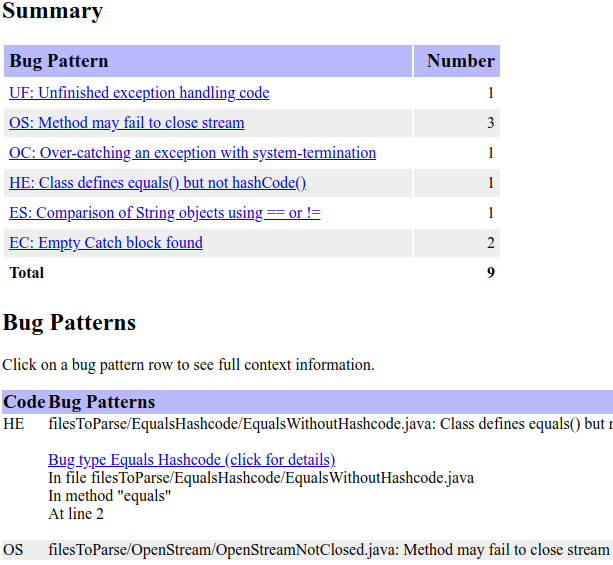
\includegraphics[width=0.4\textwidth]{report}
\caption{Excerpt of a report}
\label{report}
\end{figure}

\section{Test Cases}
Each bug pattern has two unit tests in the test folder that ensures the bug pattern is well detected when it is present in a dummy Java class and that it is not detected when a class does not exhibit the bug pattern.\\In listing \ref{lst:unittest}, a unit test class is shown, it is similar for other bug patterns. When the bug is found, the bug pattern list is checked for size (number of defects found), the file name is verified, the function name is verified as well, and we make sure that the line number is correct.
\newpage
\begin{lstlisting}[caption={Excerpt of the \texttt{TestEmptyCatch} class to unit test the \texttt{EmptyCatchClauseChecker}},captionpos=b,label={lst:unittest}]
public class TestEmptyCatch {
	@Test
    /**
    * Here we test for the empty catch clause bug
    * The EmptyCatch class contain the bug pattern,
    * so the bug checker returns one instance of the bug
    **/
	public void testEmptyCatchEmpty() {
		List<BugPattern> bugPatterns = new EmptyCatchClauseChecker().check(new File("filesToParse/.../EmptyCatch.java"));
		Assert.assertEquals(1, bugPatterns.size());
		Assert.assertEquals("EmptyCatch.java", bugPatterns.get(0).getFilename());
		Assert.assertEquals("testCatchBlock", bugPatterns.get(0).getFunctionName());
		Assert.assertEquals(9, bugPatterns.get(0).getLine());
	}
    /**
    * The bug pattern is not present in the NotEmptyCatch class,
    * so nothing should be returned
    **/
	@Test
	public void testEmptyCatchNotEmpty() {
		List<BugPattern> bugPatterns = new EmptyCatchClauseChecker().check(new File("filesToParse/.../NotEmptyCatch.java"));
		Assert.assertEquals(0, bugPatterns.size());
	}
}
\end{lstlisting}
\vspace{-3mm}

\section{Detection Results}
We run our tool and FindBugs on CloudStack 4.9 and Hadoop 3.0.0.
\subsection{Running Our Tool}
To run our tool, we extracted the zip files of CloudStack and Hadoop at the root of our tool, next to the filesToParse folder. Then, we modified the following line from the Main.java file, to change the default folder to CloudStack's and Hadoop's. This is shown in listing \ref{lst:mainfolder}.
\begin{lstlisting}[caption={Excerpt of the \texttt{Main} class that defines the folder to parse},captionpos=b,label={lst:mainfolder}]
File projectDir = new File("filesToParse");
\end{lstlisting}
\vspace{-3mm}
At the end of the analysis, an HTML result file is generated. We faced scalability issues: since we only tried our project with a few classes, scaling from a dozen of classes to thousands of them was not trivial. We had to improve our checkers so they are more efficient memory-wise, and we have to raise the Java heap using the -Xmx argument. Memory usage has been reduced using a method's hashcode instead of the \texttt{MethodDeclaration} instance. We had to raise it to 9GB of RAM to make it work for Hadoop. Table \ref{toolresult} shows the results for our tool on on CloudStack 4.9 and Hadoop 3.0.0.
\begin{table}[ht!]
\begin{tabular}{|l|l|l|}
\hline
\textbf{Bug Pattern}                                                                                 & \textbf{Hadoop} & \textbf{CloudStack} \\ \hline
\begin{tabular}[c]{@{}l@{}}UF: Unfinished exception\\ handling code\end{tabular}                     & 34                    & 102                     \\ \hline
\begin{tabular}[c]{@{}l@{}}IL: Duplicate logging statements\\ in different catch blocks\end{tabular} & 5                     & 2                       \\ \hline
\begin{tabular}[c]{@{}l@{}}OC: Over-catching an exception\\ with system-termination\end{tabular}     & 13                    & 48                      \\ \hline
\begin{tabular}[c]{@{}l@{}}OS: Method may fail\\ to close stream\end{tabular}                        & 51                    & 17                      \\ \hline
\begin{tabular}[c]{@{}l@{}}UM: The method is defined\\ but never used\end{tabular}                   & 23,974                 & 21,899                   \\ \hline
IC: Condition is ineffective                                                                         & 3                     & 6                       \\ \hline
\begin{tabular}[c]{@{}l@{}}HE: Class defines equals()\\ but not hashCode()\end{tabular}              & 8                     & 4                       \\ \hline
EC: Empty Catch block found                                                                          & 1,645                  & 83                      \\ \hline
\begin{tabular}[c]{@{}l@{}}UC: Uneeded computation\\ is present in a loop\end{tabular}               & 917                   & 89                      \\ \hline
\begin{tabular}[c]{@{}l@{}}ES: Comparison of String\\ objects using == or !=\end{tabular}            & 2                     & 2                       \\ \hline
Total number of bugs found                                                                                       & 26,652                 & 22,252                   \\ \hline
\end{tabular}
\caption{Bug detection result for our tool on Hadoop and CloudStack}
\label{toolresult}
\vspace{-10mm}
\end{table}

\subsection{Running FindBugs}
Next, we run FindBugs on Hadoop 3.0.0 and CloudStack 4.9. Both projects are from the Apache foundation and follow the same guidelines. To analyze bugs, we had to build and compile the two projects. We faced some issues doing so, for example we had to install Protobuf 2.5.0 otherwise Hadoop would not compile with a later version \cite{buildinghadoop}. Then, one can run the compilation and FindBugs report generation with the following command described in listing \ref{lst:mavenfindbugs}.
\begin{lstlisting}[caption={Maven command to run FindBugs generation},captionpos=b,label={lst:mavenfindbugs}]
mvn compile findbugs:findbugs
\end{lstlisting}
\vspace{-3mm}
This command makes FindBugs generate a \texttt{findBugsXml.xml} file for each subproject. This means that we have to merge them together, and this can be done using an undocumented option, UnionBugs \cite{unionbug}. Then, the merged XML file can be opened in FindBugs or SpotBugs, and a HTML or TXT report can be generated.
Then, we found that Hadoop only had one bug, which does not seem realistic given the size of the project. Later, we found that the development team had FindBugs ignore bugs using XML filter files. We replaced those files with an empty filter to get the full report, since our tool does not implement a filter feature. The same files were present in CloudStack but applying the same process did not change the result output. We found that for Hadoop and CloudStack, SpotBugs was not supported and only FindBugs was available. Table \ref{findbugsresult} shows the results of the FindBugs analysis.

\vspace{-3mm}
\begin{table}[ht!]
\begin{tabular}{|l|l|l|}
\hline
\textbf{Project}                                                                          & \textbf{Hadoop} & \textbf{CloudStack} \\ \hline
Lines of code                                                                             & 943,502               & 318,866                 \\ \hline
Number of classes                                                                         & 14,564                & 5,800                   \\ \hline
Number of packages                                                                        & 546                   & 473                     \\ \hline
Number of bugs                                                                            & 2,945                 & 127                     \\ \hline
\begin{tabular}[c]{@{}l@{}}HE\end{tabular}   & 0                     & 0                       \\ \hline
\begin{tabular}[c]{@{}l@{}}ES\end{tabular} & 2                     & 0                       \\ \hline
\begin{tabular}[c]{@{}l@{}}OS\end{tabular}             & 1                     & 0                       \\ \hline
IC                                                              & 0                     & 0                       \\ \hline
\end{tabular}
\caption{Bug detection result for FindBugs on Hadoop and CloudStack}
\label{findbugsresult}
\vspace{-10mm}
\end{table}
\noindent Most bugs (91\%) found in CloudStack were internationalization warnings, meaning that methods would "perform a byte to String conversion, and will assume that the default platform encoding is suitable", possibly causing unwanted behaviors depending on the platform.

\subsection{Comparing the Results}
The table \ref{tablerecap} sums up the differences for bug patters 1 to 4 between our solution and FindBugs.

\begin{table}[ht!]
\begin{tabular}{|l|l|l|l|l|}
\hline
Tool    & \multicolumn{2}{c|}{Our Tool} & \multicolumn{2}{c|}{FindBugs} \\ \hline
Project & Hadoop      & CloudStack      & Hadoop      & CloudStack      \\ \hline
HE      & 8           & 4               & 0           & 0               \\ \hline
ES      & 2           & 2               & 2           & 0               \\ \hline
OS      & 51          & 17              & 1           & 0               \\ \hline
IC      & 3           & 6               & 0           & 0               \\ \hline
\end{tabular}
\caption{Recapitulating the bug number difference}
\label{tablerecap}
\vspace{-10mm}
\end{table}

\begin{enumerate}
    \item HE - Class defines \texttt{equals} but not \texttt{hashCode}: our tool scoped to the current class only, so that if a class defines a \texttt{hashCode} function in the parent class and \texttt{equals} in the child class, it will report a bug. This is the case for the \texttt{RMDelegationToken\-IdentifierForTest} class: it extends the \texttt{RMDelegation\-TokenIdentifier} class which extends \texttt{YARNDelegation\-TokenIdentifier}, which extends \texttt{AbstractDelegation-}\newline\texttt{TokenIdentifier} that finally implements \texttt{hashCode}.
    \item ES - Comparison of \texttt{String} objects using == or !=: the two bugs detected by our tool in CloudStack should have been detected by FindBugs. Listings \ref{lst:es1} and \ref{lst:es2} show what has been detected by our tool:
\begin{lstlisting}[caption={Excerpt from the \texttt{Script} class, definition of the \texttt{ERR\_TIMEOUT} attribute},captionpos=b,label={lst:es1}]
public static final String ERR_TIMEOUT = "timeout";
\end{lstlisting}
\vspace{-5mm}
\begin{lstlisting}[caption={Excerpt from the \texttt{KVMHABase} class, method \texttt{runScriptRetry} in the CloudStack hypervisors KVM plugin},captionpos=b,label={lst:es2}]
String result = null;
...
if (result == Script.ERR_TIMEOUT) { // should not be done!
\end{lstlisting}
\vspace{-3mm}
Here, the \texttt{result} variable, which is a \texttt{String}, is compared with the equality operator against the \texttt{Script.ERR\_TIMEOUT} variable, also being a \texttt{String}.
    \item OS - Method may fail to close stream on exception: the difference is coming from the fact that our tool has a scope limited to the current method to check if the stream has been closed in the \texttt{finally} block. For example, the code in listing \ref{lst:openstream} is closing the stream without using the \texttt{close} function directly. Thus, our tool detects a bug because the stream is not explicitly closed within the function.
\begin{lstlisting}[caption={Excerpt from the \texttt{DebugAdmin} class, method \texttt{run} in the Hadoop HDFS project},captionpos=b,label={lst:openstream}]
finally {
    IOUtils.cleanup(null, metaStream, dataStream, checksumStream);
}
\end{lstlisting}
\vspace{-3mm}
    \item IC - Condition has no effect: our tool detected real bug patterns in CloudStack, such as shown in listing \ref{lst:upgrade} in the \texttt{DatabaseUpgradeChecker} class:
\begin{lstlisting}[caption={Excerpt from the \texttt{DatabaseUpgradeChecker} class, method \texttt{upgrade} in the upgrade CloudStack package},captionpos=b,label={lst:upgrade}]
if (true) { // FIXME Needs to detect if management servers are running
\end{lstlisting}
\vspace{-3mm}
We do not know why this was not detected by FindBugs after the removal of the FindBugs filter.
\end{enumerate}

\section{Threats to Validity}
Our study only focused on analyzing only two softwares: CloudStack and Hadoop. There is no certainty that those findings could be generalized to other software. We have no software to compare the results to for bugs 5 to 10.

\section{Related Work}
The FindBugs software has been described by Nathaniel Ayewa et al. in 2008 \cite{ayewah}. In 2011, Antonio Vetro et al. have discussed about the validation of FindBugs issues \cite{vetro_morisio_torchiano_2011}.

\section{Future Work}
The findings of the paper could be extended by redoing the tests on SpotBugs. Additional software could be tested. Our solution could be improved to scale better for larger software.

\section{Conclusion}
In this paper, we created a software that is able to detect 10 different bugs patterns. We run this tool on two open source software, Hadoop 3.0.0 and CloudStack 4.9. We compared the results with the results obtained from running FindBugs on those two software for the common bug patterns. We found that the differences we observed were due to either a reduced scope in our software or a lack of detection in FindBugs.

\begin{acks}
We would like to thank our supervisor, Dr. Tse-Hsun (Peter) Chen, for the patient guidance, encouragement and advice he has provided throughout the duration of the project.
\end{acks}

\bibliographystyle{ACM-Reference-Format}
\bibliography{bibliography}

\end{document}
